\chapter{Aprendizado de Máquina}
\label{chap:cap1}
 
 O aprendizado de máquina é uma área da inteligência artificial que possui o objetivo de desenvolver técnicas e algoritmos que permitam ao computador adquirir conhecimento a partir de amostras, e assim aperfeiçoar seu desempenho em uma determinada tarefa.\cite{goldschmidt}
 
 Uma amostra pode ser descrita como um grupo de atributos que juntos descrevem um objeto de interesse. Como exemplo, pode ser considerado o histórico médico de um paciente, onde seus atributos seriam o conjunto de dados relevantes que compõem o histórico.
 
 Os algoritmos de aprendizado de máquina adquirirem conhecimento através do processo de indução, que é o processo de inferência lógica que permite obter conclusões genéricas sobre um conjunto particular de amostras. Por exemplo, um algoritmo que recebesse o histórico de compras de um grupo de pessoas poderia criar hipóteses, através da indução, sobre quais produtos elas são mais propensas a comprar. É importante ressaltar que as hipóteses geradas pelos algoritmos nem sempre são verdade.\cite{Monard2003a}
 
 O aprendizado indutivo pode ser dividido em supervisionado e não supervisionado. \cite{Monard2003a}
 

\section{Aprendizado Supervisionado}
\label{sec:superv}

 No aprendizado supervisionado, um sistema é treinado com uma base de dados de amostras compostas de um conjunto de valores de características, ou atributos, que servem como entrada do sistema e um conjunto de rótulos que são a melhor saída possível para a entrada respectiva. 
 
 Comparando a saída do sistema para cada atributo com o rótulo correspondente, um sinal de erro é calculado e utilizado iterativamente para adaptar o sistema de aprendizagem. Analogamente, a saída do sistema comparada à saída esperada e conhecida (o rótulo), auxilia o sistema a se aperfeiçoar. Desse modo, conforme o treino é realizado, o sistema se aproxima cada vez mais do modelo do ambiente descrito pelas amostras. 
 
 O objetivo desta classe de algoritmo descrita é gerar classificadores capazes de determinar os rótulos de atributos ainda não classificados.\cite{haykin2009neural, goldschmidt} Na Figura \ref{fig:supervisionado} é mostrado o diagrama de aprendizado supervisionado.
 
 \begin{figure}[htb]
 \caption{\label{fig:supervisionado} Diagrama do aprendizado supervisionado}
 \begin{center}
 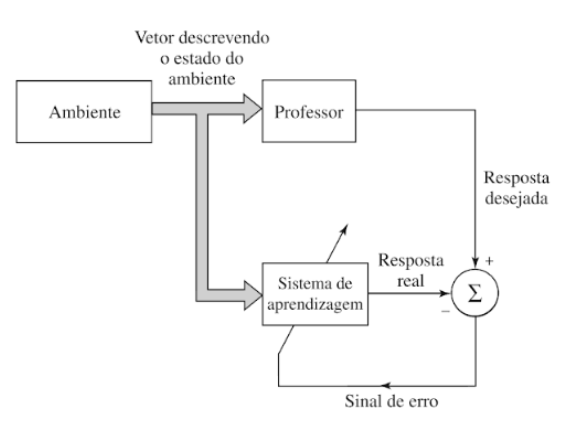
\includegraphics[scale=0.5]{AprendizadoSupervisionado}
 \end{center}
 \legend{Fonte: \citeauthor{haykin2009neural}, \citeyear{haykin2009neural}} 
 \end{figure}
 
 Nesta classe de algoritmos há uma diferente dissociação entre aqueles que lidam com rótulos discretos, cujos problemas são conhecidos como classificação, e aqueles que lidam com rótulos contínuos, cujos problemas são conhecidos como regressão. 
 
 Nos problemas de classificação, o objetivo é classificar as entradas em categorias. Por exemplo, um sistema que distingue o modelo de carros baseado em fotos. Para problemas de regressão, os resultados obtidos do sistema formam uma função contínua. Um exemplo seria um sistema que calcula o valor de uma moeda nos próximos 30 dias baseado na sua flutuação durante o mês anterior. Na Figura \ref{fig:classregres} é apresentado um exemplo conceitual da diferença entre classificação e regressão.
 
 \begin{figure}[htb]
 \caption{\label{fig:classregres} Distribuição de dados de classificação e regressão}
 \begin{center}
 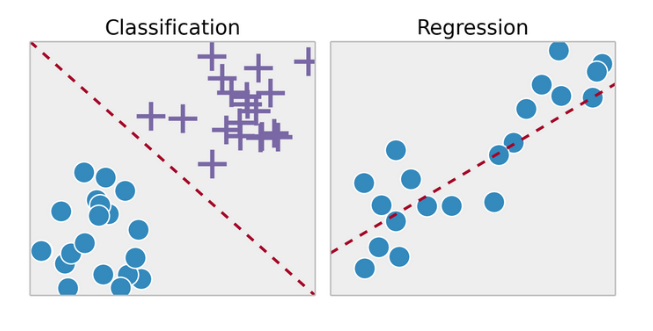
\includegraphics[scale=0.75]{ClassificacaoRegressao}
 \end{center}
 \legend{Fonte: \citeauthor{mediummachine}, \citeyear{mediummachine}} 
 \end{figure}


\section{Aprendizado Não Supervisionado}
\label{sec:nsuperv}

 No aprendizado não supervisionado o sistema é treinado com amostras não necessariamente rotulados e sem conhecimento da melhor saída possível \cite{haykin2009neural}. Por isso, a adaptação é feita a partir de uma medida independente da tarefa que mede a qualidade da representação do que o sistema deve aprender \cite{beckerneural}, por não ser possível realizar comparações com a resposta ideal para se determinar um erro. 

 Por exemplo no método de agrupamento, o sistema analisa as amostras fornecidas e as separa em grupos baseado em propriedades semelhantes encontradas. Este tipo de aprendizado é aplicável à problemas onde se deseja descobrir características relevantes nos dados de entrada \cite{goldschmidt}, porém os grupos não necessariamente apresentam informações relevantes, muitas vezes precisando de um estudo para verificar sua validade.\cite{Monard2003a} 

 Um exemplo de aplicação de técnicas de agrupamento é um sistema que analisa informações sobre vários pacientes de um hospital para tentar descobrir novos sintomas para uma determinada doença, que posteriormente são estudados por um médico para verificar se a doença em caso realmente têm relação com os sintomas encontrados.

 Na Figura \ref{fig:comparacaoaprendizado} é representado um exemplo da diferença entre o aprendizado supervisionado e não supervisionado, onde o supervisionado classifica cada saída com um rótulo e o não supervisionado agrupa as saídas de acordo com padrões. 


 \begin{figure}[htb]
 \caption{\label{fig:comparacaoaprendizado} Comparaçao entre aprendizados}
 \begin{center}
 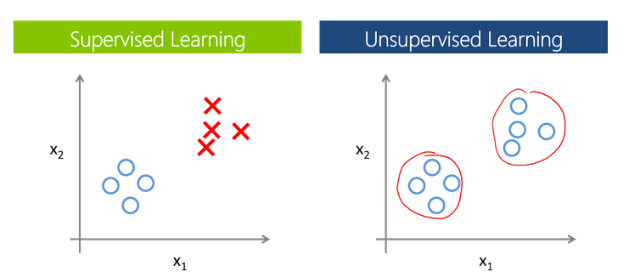
\includegraphics[scale=0.75]{ComparaAprendizado}
 \end{center}
 \legend{Fonte: \citeauthor{mediummachine}, \citeyear{mediummachine}} 
 \end{figure}

%\autoref{chap:cap1}
% ---
%\section{Aliquam vestibulum fringilla lorem}
%\lipsum[2]
%\subsection{Subsessão cap 1}
%\lipsum[2]
%\chapter{Capitulo Segundo}
%\lipsum[2]
